\subsection{Database Arkitektur}
Systemets database vil stå for at opbevare data for brugerne, dette vil være i form af data indeholdt i et gemt spil.\\
I oprettelsen af systemets database skal der tages hånd om, hvordan kommunikationen skal foregå imellem systemets segmenter, samt databasens funktionalitet. Her er der blevet besluttet at der anvendes en DAL, der fungerer ved at hver gang databasen skal kontaktes, så foregår det igennem denne. Yderligere vil denne DAL også simplificere kommunikationen mellem databasen og Back-end'en. 

\noindent Herunder vises et eksempel på hvordan kommunikationen ville foregå med databasen.

\begin{figure}[H]
\centering
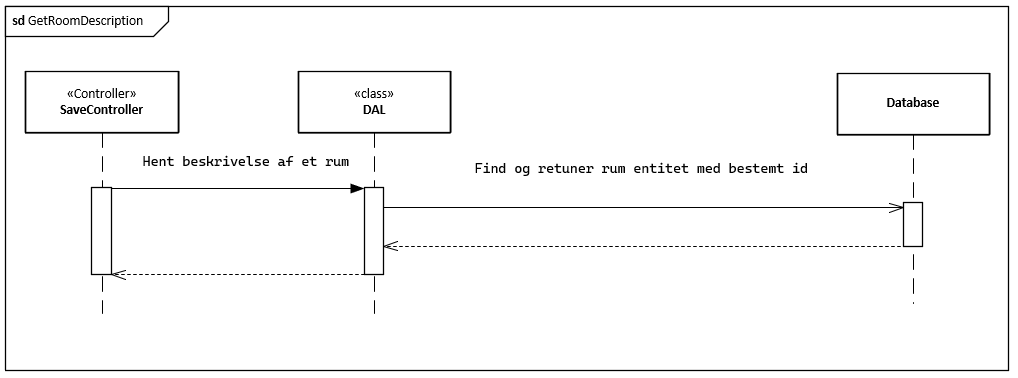
\includegraphics[width = \textwidth]{02-Body/Images/RoomDescriptionsDB.PNG}
\caption{Sekvensdiagram for hvordan rum beskrivelser vil blive hente fra databasen af SaveController}
\label{fig:RoomDescriptionsDB}
\end{figure}

\noindent I \autoref{fig:RoomDescriptionsDB} ses diagrammet GetRoomDescription ses der, hvordan kommunikationen ville foregå for at hente rum beskrivelsen. Her ses der at SaveController, fra Back-End, går til DAL, som så henter rum beskrivelsen fra databasen, og herefter returneres dataene fra databasen til DAL og så fra DAL til SaveController.

Yderligere eksempler og forklaringer vedr. kommunikation kan findes i teknisk bilag \textbf{MANGLER REF HER}

\subsubsection{DAL Arkitektur}
Når data enten skal sendes til eller hentes fra databasen så er det igennem et DAL. Systemets DAL fungerer som en mellemmand for systemet, da alt kommunikation til og fra databasen går igennem den.\\
\noindent I dette DAL vil data for at gemme et spil og indlæse et spil blive sendt igennem. Begge af disse vil indeholde det samme type data, dog ville den ene, LoadGame, hente data fra systemets database, og den anden, SaveGame, vil sende data til systemets database. 
LoadGame, og SaveGame, i DAL vil være ansvarlig for at hente spillerens data fra databasen, såsom hvilket rum de var i og mængden af liv de har tilbage.